He-like triplets, occur when the excited states of a two-electron atomic species (i.e. He-like), decay to the ground state, resulting in resonance (\textit{r}), intercombination (\textit{i}), and forbidden (\textit{f}) lines. The line strength ratios between these three lines are a function of the temperature and density of the plasma from which they arise \citesomething{}. Specifically, the forbidden transition will only occur in low density plasma \citep[e.g.][]{ness_helium-like_2001}, since in higher density plasma collisional interactions will dominate over the very rare transition. Thus, the ratio between the forbidden and intercombination lines is a useful density indicator. Similarly, the ratio between the forbidden, intercombination, and resonance line can be used to probe the temperature of the emitting plasma \citep[e.g.][]{schneider_multiepoch_2018}.

We fit the He-like triplets of Ne IX, at $\sim13.5$ \AA, using the RGS spectra. To describe the triplet we used a Gaussian triplet model, added to the plasma model used in the global fit (see above). The Gaussian triplet model consists of three coadded gaussian profiles. It is described by seven parameters: the positions of each component, $pos_i, pos_r, pos_f$, the fwhm of an emission line, fwhm, the amplitude of the intercombination component, $amp_i$, and the R-ratios and G- ratios, defined by \citet{pradhan_density_1981} as: 
\begin{equation}
    R = f/i
\end{equation}
\begin{equation}
    G = (f+i)/r
\end{equation}
To fit the triplet we locked all plasma model parameters to the best-fit values from the global fit (see Table \ref{table:global_fit}), with the exception of Ne, which we locked to an abundance of zero so that it could be fully fit by the triplet component of the model. We also locked the positions and fwhm of the triplet components, allowing only the amplitude and ratios to vary. We performed the fit independently for the two epochs of data.

There are several Fe emission lines close to the $r$ and $i$ components of the Ne triplet. At the resolution of the RGS we are unable to distinguish between the Ne IX resonance line and the Fe XIX line, which may ``contaminate" the line ratios. To mitigate this we use the plasma model along with the triplet model, where the plasma model includes the Fe emission lines, but the Ne lines are fit only by the triplet model. Additionally, our global fit shows that, like other classical T-Tauri's, the Ne abundance in SU Aur is significantly above solar, while the Fe abundance is solar or sub-solar, so the emission from the Fe lines should be relatively weaker than that from Ne \citep[e.g.][]{gunther_disk-bearing_2010}.

\begin{figure}
    \centering
    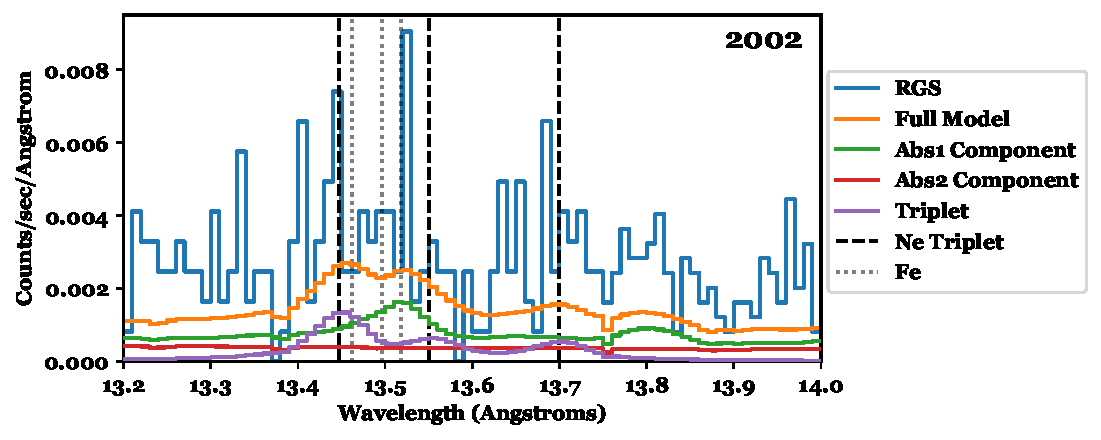
\includegraphics[width=0.98\linewidth]{Figures/SU Aur/figure_ne_triplet_fit_2002.pdf}
    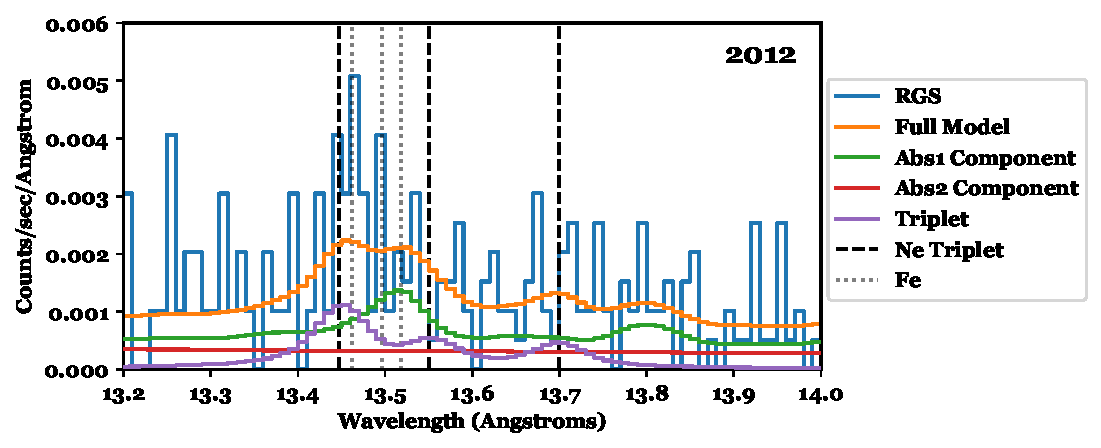
\includegraphics[width=0.98\linewidth]{Figures/SU Aur/figure_ne_triplet_fit_2012.pdf}
    \caption{The fit to the RGS spectra of the Ne He-like triplet at $13.5$\AA. The 2002 data is shown on top and the 2012 data on the bottom. The locations of the $r, i, $ and $f$ Ne triplet components are marked with solid black dashed lines, and the locations of nearby Fe lines with faint gray lines. The Fe line at $13.462$ is particularly close to the Ne $r$ component at $13.4473$, and may be producing blended contamination. The model fits are overplotted as colored lines on the data, in which the orange line is the full model, the red and green lines are the two components of the XSPEC plasma model, and the purple line is the Gaussian triplet model. At this wavelength the primary plasma model contribution comes from the first, higher absorbing column density, absorption component and its two temperature components.}
    \label{fig:ne_triplet}
\end{figure}

Fitting the 2002 epoch, we find that the best fit results are  $R_{obs} = 4.69\pm24.7$ and $G_{obs}=1.41\pm0.15$. This G-ratio suggests a plasma temperature of $log(T)\approx6.0$. The R-ratio is too unconstrained to place limits on the temperature, but is consistent with the low-density limit, $log(n_e) < 10.5$, although we cannot rule out a high-density scenario at $1\sigma$ confidence.

For the 2012 data we find best fit ratios of $R_{obs}=0.96\pm2.11$ and $G_{obs} = 0.75 \pm nan$. Both of these are relatively unconstrained due to the low number of counts in the Ne triplet region of the 2012 RGS spectrum. We are therefore unable to place limits on the temperature of the emitting plasma using the G-ratio. Regardless of temperature, the $R$-ratio suggests a higher density than the 2002 epoch, with a $1\sigma$ confidence limit of $log(n_e) > 10.5$.

Overall, while the low counts in the Ne IX triplet region limit the statistical significance of our results, we find that in 2002 the best fit to triplet emitting plasma is consistent with having a low temperature, $T\approx1\times10^6 K$, and a low density, while the 2012 results suggest a potentially higher density.

% - - - - - - - - - - - - - - - - - - - - - - - - - - - - - - - - - - - - - - - - 

We use the individual line fits to probe the temperature and absorbing column density of the emitting plasma independently from the global plasma fit. The flux ratio between the Lyman $\alpha$ and $\beta$ lines of each species is a probe of temperature and absorbing column density. 
We use CHIANTI models of line emission as a function of temperature combined with an XSPEC absorption model (\textit{phabs}), to determine the sensitivity to temperature and absorbing column density.
We calculate the line ratios for each Lyman $\alpha$ and $\beta$ set, and compare them to the model.

In the 2002 and 2012 quiescent spectra, O XIII has a Ly $\alpha/\beta$ ratio of $1.28$ and $0.77$, respectively. This low ratio requires a high absorbing density, $N_H > 0.9 10^{22} cm^{-2}$. 
In contrast, the Ne X Ly $\alpha/\beta$ ratio is \red{$13.69$} (2002) and $8.84$ (2012), indicating a much lower absorbing density, with an upper limit of $N_H < 0.5 10^{22} cm^{-2}$ at temperatures greater than $1\times10^7$ K, lower than our temperature component. 
This suggests that the Oxygen and Neon lines are being emitted from two different regions with different column absorption densities, supporting the two-absorption component model found through the global fit.